\documentclass{article}
\usepackage{graphicx}
\usepackage{amsmath}
\usepackage{float}

\title{Performance Comparison of Linear SVM, Gaussian SVM, and Neural Network}
\author{Isaak Wiebe, V01004501}
\date{\today}

\begin{document}

\maketitle

\section{Introduction}
This report presents the performance evaluation of three machine learning models: Linear Support Vector Machine (SVM), Gaussian Kernel SVM, and a Neural Network. The models were trained and tested on the MNIST fashion dataset with a focus on optimizing hyperparameters through cross-validation. The results are analyzed through various performance metrics, including test error and confidence intervals.

\section{Methodology}

\subsection{Data Preprocessing}
To ensure optimal model performance, the dataset was first normalized. The binary classification task was then set up, followed by the application of the \texttt{normalize} function from scikit-learn to scale the data. Additionally, noise was intentionally added to the dataset to increase the difficulty of the classification problem and improve model robustness.

\subsection{Model Training and Hyperparameter Tuning}

\subsubsection{Linear Support Vector Machine (SVM)}
A linear SVM was trained, with the regularization parameter $C$ optimized via cross-validation. The optimal $C$ value was selected based on the highest validation accuracy.

\subsubsection{Gaussian Support Vector Machine (SVM)}
A Gaussian Kernel SVM was trained, where both the regularization parameter $C$ and the kernel coefficient $\gamma$ were tuned using cross-validation to identify the best performing configuration.

\subsubsection{Neural Network}
A 3-layer neural network was trained, with hyperparameters such as the number of hidden layers, activation functions, and epochs systematically varied to determine the optimal configuration.

\section{Results}

\subsection{Linear SVM Performance}
Figure \ref{fig:svm_c} illustrates the relationship between the regularization parameter $C$ and cross-validation accuracy. Figure \ref{fig:svm_error} shows a comparison of training and test errors across different $C$ values.

\begin{figure}[H]
    \centering
    \includegraphics[width=0.8\textwidth]{crossval_accuracy_C.png}
    \caption{Cross-validation accuracy as a function of the regularization parameter $C$ for a Linear SVM. The plot illustrates how varying $C$ affects the model's ability to generalize, with higher values of $C$ reducing regularization and potentially leading to overfitting. The optimal value of $C$ balances bias and variance to maximize cross-validation accuracy.}
    \label{fig:svm_c}
\end{figure}

\begin{figure}[H]
    \centering
    \includegraphics[width=0.8\textwidth]{training_test_error_C.png}
    \caption{Training and test error as a function of the regularization parameter $C$ for a Linear SVM. The plot highlights the trade-off between training error and test error as $C$ varies. Lower values of $C$ increase regularization, potentially underfitting the data, while higher values may lead to overfitting, as indicated by the divergence between training and test errors.}
    \label{fig:svm_error}
\end{figure}

\subsection{Gaussian SVM Performance}
Figure \ref{fig:gaussian_gamma} displays cross-validation accuracy against different $\gamma$ values for a Gaussian SVM. The kernel coefficient $\gamma$ controls the influence of individual training samples, with smaller values resulting in a smoother decision boundary and larger values capturing finer details of the data.

\begin{figure}[H]
    \centering
    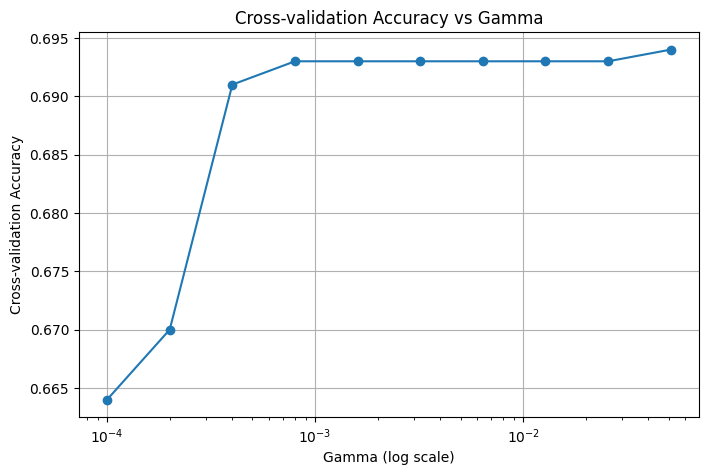
\includegraphics[width=0.8\textwidth]{crossval_accuracy_gamma.png}
    \caption{Cross-validation accuracy as a function of the kernel coefficient $\gamma$ for a Gaussian SVM. The plot demonstrates how $\gamma$ impacts model performance, with an optimal value balancing the trade-off between underfitting and overfitting. Extremely high values of $\gamma$ may lead to overfitting, while very low values may result in underfitting.}
    \label{fig:gaussian_gamma}
\end{figure}

\subsection{Neural Network Performance}
Figures \ref{fig:nn_nodes} and \ref{fig:nn_epochs} illustrate the impact of varying the number of hidden nodes and training epochs, respectively, on the performance of a Neural Network.

\begin{figure}[H]
    \centering
    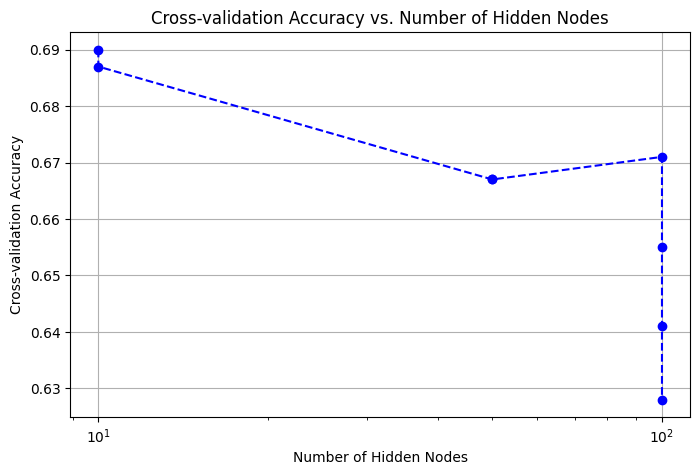
\includegraphics[width=0.8\textwidth]{crossval_accuracy_hidden_nodes.png}
    \caption{Cross-validation accuracy as a function of the number of hidden nodes in a Neural Network. The plot shows how increasing the number of hidden nodes affects the model's capacity to learn complex patterns. However, too many nodes may lead to overfitting, while too few may result in underfitting.}
    \label{fig:nn_nodes}
\end{figure}

\begin{figure}[H]
    \centering
    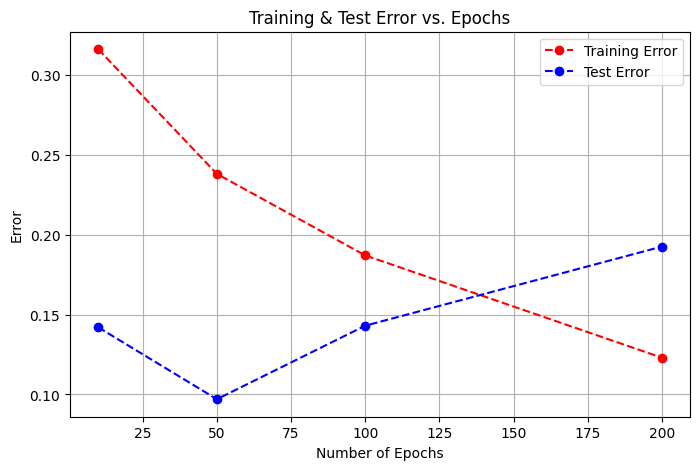
\includegraphics[width=0.8\textwidth]{training_test_error_epochs.png}
    \caption{Training and test error as a function of the number of epochs in a Neural Network. The plot highlights the relationship between training duration and model performance. Early stopping may be necessary to prevent overfitting, as indicated by the divergence between training and test errors at higher epochs.}
    \label{fig:nn_epochs}
\end{figure}

\subsection{Final Model Comparison}
The final test errors for all models are shown in Figure \ref{fig:final_comparison}, providing a comprehensive comparison of their generalization performance.

\begin{figure}[H]
    \centering
    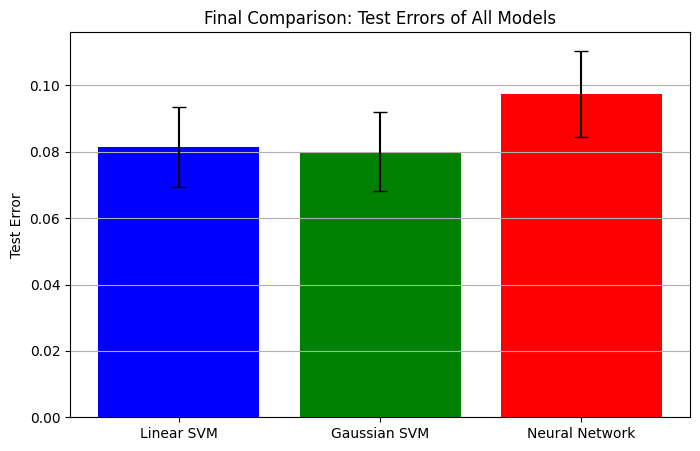
\includegraphics[width=0.8\textwidth]{test_error_comparison.png}
    \caption{Comparison of test errors for Linear SVM, Gaussian SVM, and Neural Network. The plot summarizes the generalization performance of each model, highlighting their relative strengths and weaknesses. The Gaussian SVM demonstrates improved generalization over the Linear SVM, while the Neural Network achieves competitive performance, suggesting its suitability for complex datasets.}
    \label{fig:final_comparison}
\end{figure}

\section{Conclusion}
From the results, we observe that the Gaussian SVM provided improved generalization over the Linear SVM, while the Neural Network demonstrated competitive performance. Further tuning and regularization strategies, such as dropout or weight decay for the Neural Network, could be explored to refine these models and enhance their generalization capabilities.

I think SVMs had a big advantage due to the fact that we changed the problem to a classification problem and my resources were limited. I would be inclined to believe, based on the results shown by neural networks, that given more resources and finer tuning they could surpass the performance of the SVMs. SVMs have shown themselves to be a powerful and rather lightweight option through these experiments.

\end{document}